\documentclass[aspectratio=169]{beamer}
   \usetheme{metropolis}
   \setbeamertemplate{blocks}[rounded][shadow=false]
\usepackage{url}
\usepackage{hyperref}
\usepackage{booktabs}
\usepackage{tabularx}
\usepackage{dcolumn}
   \newcolumntype{d}[1]{D{.}{.}{#1}}
\usepackage{graphicx}
\usepackage{adjustbox}
\usepackage{color}
\usepackage{textpos}
\usepackage{etoolbox}
\usepackage[cache=false]{minted}

\makeatletter
\patchcmd{\beamer@sectionintoc}{\vskip1.5em}{\vskip0.5em}{}{}
\makeatother

\definecolor{smured}{rgb}{0.797,0,0.027}
\definecolor{smublue}{RGB}{48,64,116}
\definecolor{dkgreen}{rgb}{0,0.6,0}
\definecolor{gray}{rgb}{0.5,0.5,0.5}
\definecolor{mauve}{rgb}{0.58,0,0.82}
\definecolor{text_gray}{RGB}{46,58,62}

\setbeamercolor{progress bar}{fg=smured,bg=smublue}
\setbeamercolor{title separator}{fg=smublue}
\setbeamercolor{frametitle}{bg=smublue}

\metroset{
  numbering=fraction
}

\hypersetup{
  colorlinks=true,
  allcolors=text_gray,
  urlcolor=smured,
}

\addtobeamertemplate{frametitle}{}{
\begin{textblock*}{1cm}(\textwidth,-1.155cm)

\includegraphics[width=1cm]{figures/smu_logo.pdf}
\end{textblock*}}

\setminted{breaklines,linenos,fontsize=\scriptsize}
\setmintedinline{fontsize=auto}

\title[Python]{Python Workflows on ManeFrame II (M2)}
\author{Robert Kalescky\\ HPC Applications Scientist \\
John LaGrone \\ HPC Research Solutions Architect }
\institute{
Research and Data Sciences Services\\
Office of Information Technology\\
Center for Research Computing\\
Southern Methodist University}
\date{\today}


\begin{document}

\begin{frame}
\titlepage
\end{frame}

\begin{frame}{Outline}
\footnotesize
\tableofcontents[hideallsubsections]
\end{frame}

\section{Research Support}

\begin{frame}{Research and Data Science Services}
\begin{itemize}
  \item Provide research computing support, consultations, and collaborations
  \item Data Science - Dr. Eric Godat
  \item High-Performance Computing - Dr. Robert Kalescky \& Dr. John LaGrone
  \item Custom Devices (IOT, wearables, etc.) - Guillermo Vasquez
\end{itemize}
\end{frame}

\begin{frame}{Center for Research Computing (CRC)}
\begin{itemize}
  \item Maintains our primary shared resource for research computing, ManeFrame II (M2), in collaboration with OIT
  \item Provides research computing tools, support, and training to all faculty, staff, and students using research computing resources
  \item \url{www.smu.edu/crc} has documentation and news
  \item \href{mailto:help@smu.edu}{help@smu.edu} or \href{mailto:rkalescky@smu.edu}{rkalescky@smu.edu} for help
  \item Request an account at \url{www.smu.edu/crc}
\end{itemize}
\end{frame}

\begin{frame}{Spring 2022 CRC HPC Workshop Series}
\begin{table}
\tiny
\begin{tabular}{lll}
Date     & Time  & Workshop\\
\hline
February 2 & 2-4 & ManeFrame II (M2) Introduction \\  
February 9 & 2-4 & Workflows in R \\  
February 15 & 3-5 & Finding and Preparing Text Data Sets for Mining \\
Febryary 16 & 1-4 & Machine Learning with Python Part 1 \\
February 17 & 12-1 & AI for the Non-Expert \\
February 18 & 12-1 & Introduction to GitHub \\        
February 23 & 2-4  & Containers and Spack \\     
March 2   &  2-4 &  ManeFrame II (M2) Introduction \\
March 3   &  1-4 & Data Science Workflow with R \\  
March 8   &  3-6 & Introduction to Python for Text Mining \\ 
March 9   &  1-4 & Machine Learning with Python Part 2 \\ 
March 22  &  3-6 & Getting Support for Text Mining \\  
March 23  &  2-4 & Shared Memory Parallelism \\   
March 30  &  1-4 & Deep Learning with Python Part 1 \\   
April 6   &  2-4 & ManeFrame II (M2) Introduction \\    
April 13  &  2-4 & Accelerator Libraries and APIs \\    
April 20  &  1-4 & Deep Learning with Python Part 2 \\      
April 27  &  2-4 & MPI/NCCL/SHMem \\            
May 4     &  2-4 & ManeFrame II (M2) Introduction      
\end{tabular}
\caption{Workshops will be held each Wednesday from 2:00 to 4:00 PM. Sessions will typically be                                
recorded and posted along with session materials.         
Register on the Library Workshop Calendar \href{https://libcal.smu.edu/calendar/libraryworkshops}{https://libcal.smu.edu/calendar/libraryworkshops}
}
\end{table}
\end{frame}

\section{ManeFrame II (M2)}

\begin{frame}{Cluster Super Computers}
\begin{figure}
  \centering
  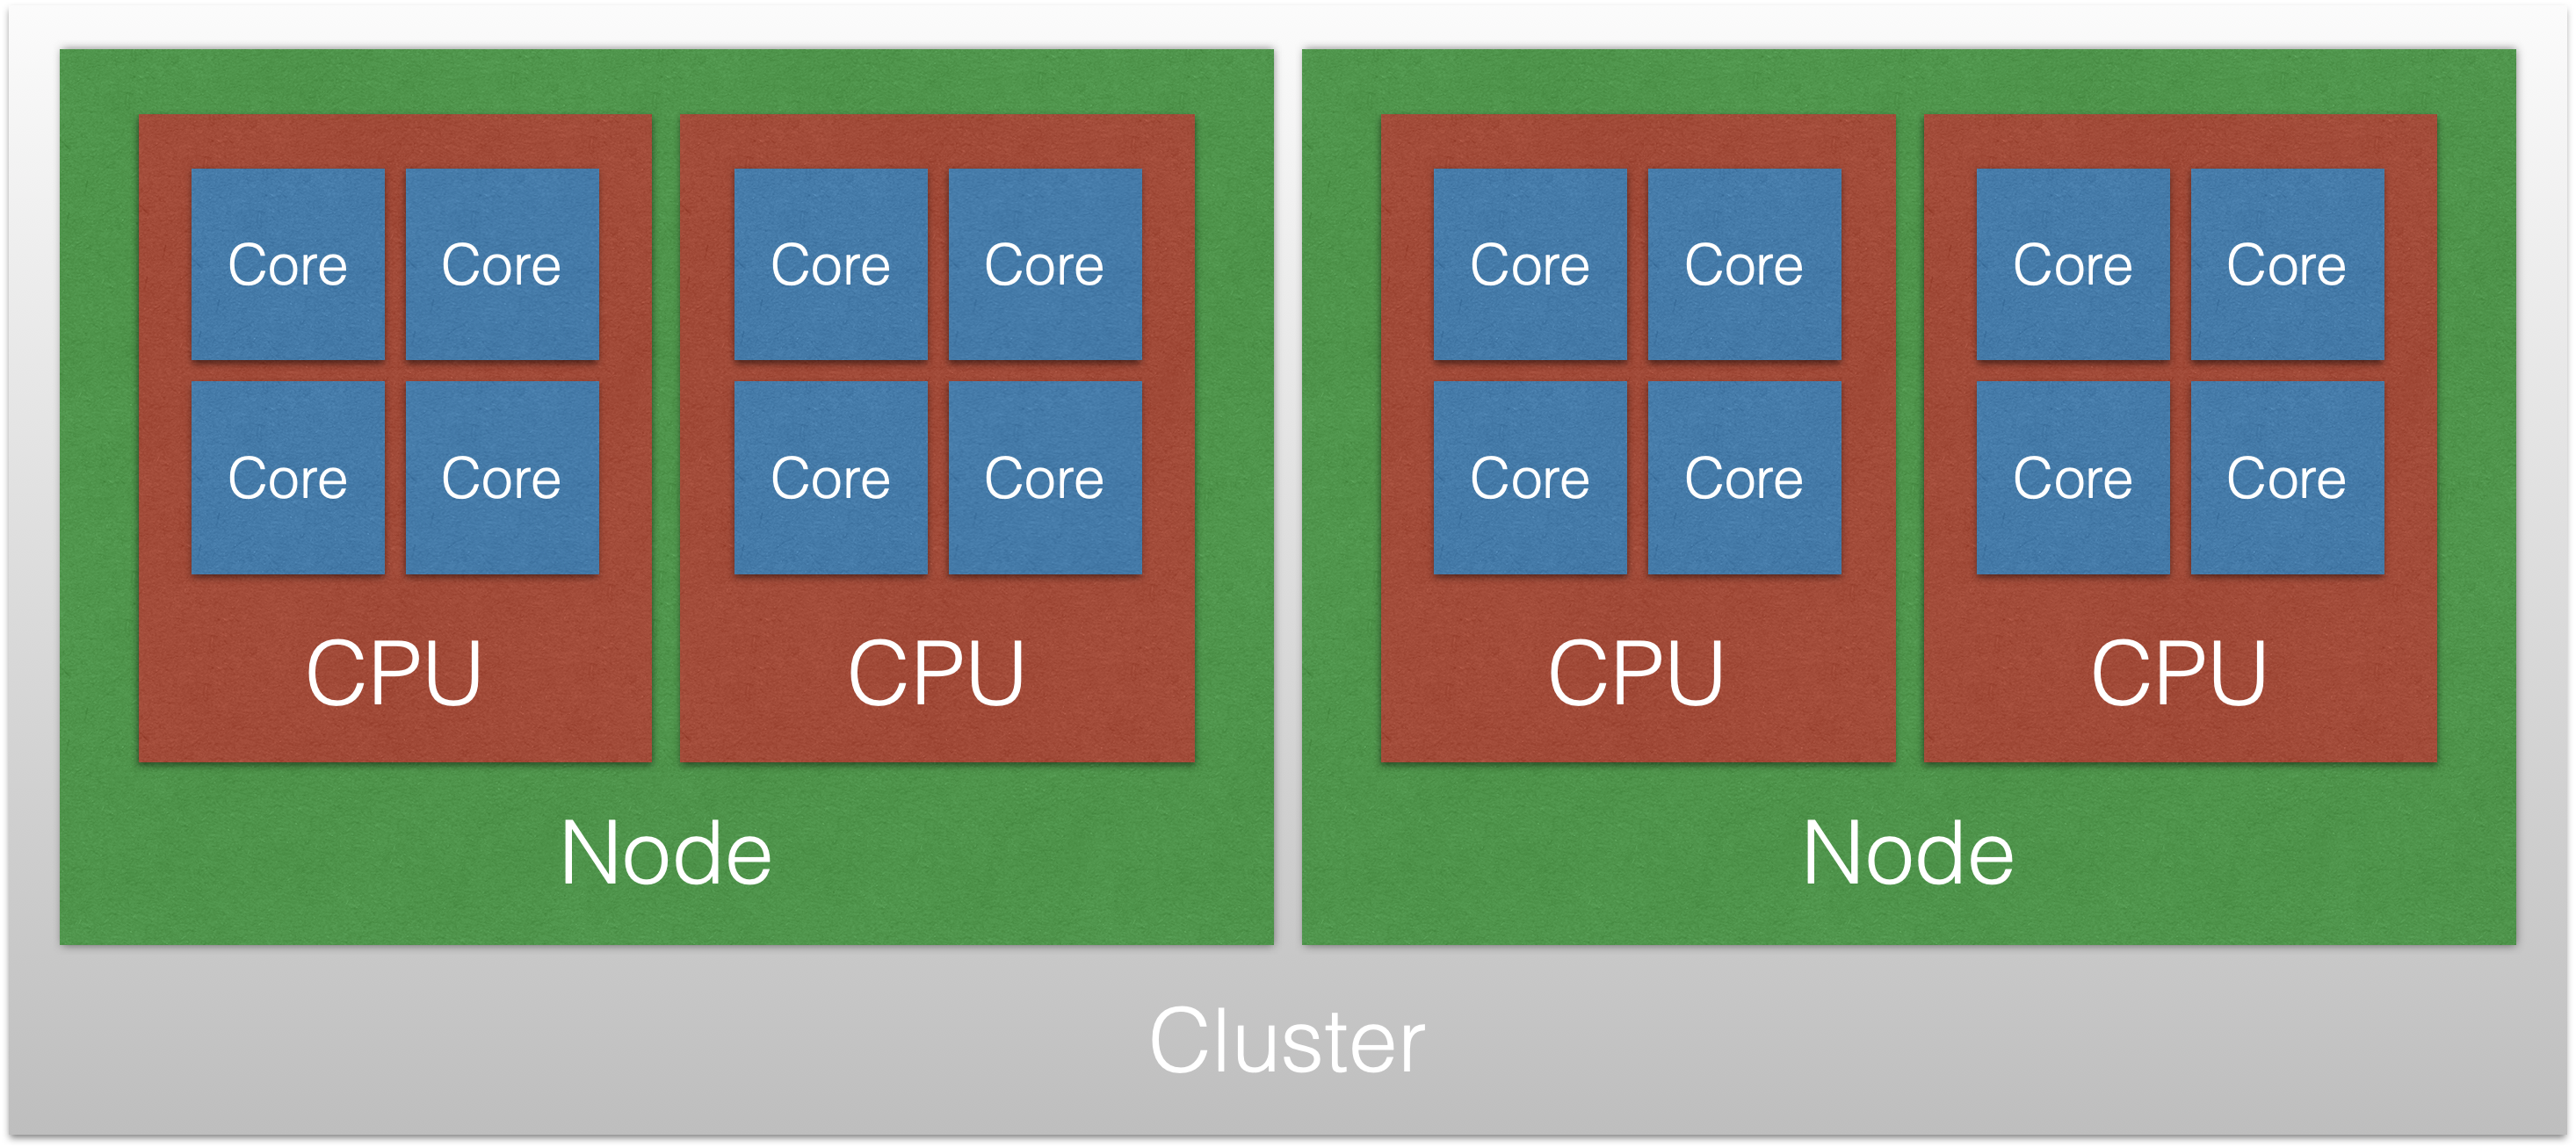
\includegraphics[width=0.75\linewidth]{figures/cluster.png}
  \caption{A cluster is a collection of individual computers networked together. Applications can be configured to run on all available compute resources.}
\end{figure}
\end{frame}

\begin{frame}{ManeFrame II (M2) Node Types}
\begin{table}
\tiny
\begin{tabular}{lllll}
\toprule
Type & Quantity & Cores & Memory [GB] & Additional Resources\\
\midrule
Standard-Memory & 176 & 36 & 256 & \\
Medium-Memory-1 & 35 & 36 & 768 & \\
Medium-Memory-2 & 4 & 24 & 768 & 3 TB SSD local scratch\\
High-Memory-1 & 5 & 36 & 1,536 & \\
High-Memory-2 & 6 & 40 & 1,536 & 3 TB SSD local scratch\\
GPGPU-1 & 36 & 36 & 256 & NVIDIA P100 GPU has 3,584 CUDA cores and 16 GB CoWoS\\
MIC-1 & 36 & 64 & 384 & 16 GB of high bandwidth (400 GB/s) stacked memory\\
VDI & 5 & 36 & 256 & NVIDIA Quadro M5000 GPU\\
v100x8 & 3 & 36 & 768 & 8 NVIDIA V100 GPUs with 5,120 CUDA cores and 32 GB CoWoS\\
Faculty Partner Nodes & 3 &  &  & Various research specific NVIDIA GPU configurations\\
\midrule
ManeFrame II & 354 & 11,276 & 120 TB & 2.8 PB storage and InfiniBand network\\
\bottomrule
\end{tabular}
\end{table}
\end{frame}

\begin{frame}{ManeFrame II (M2) Partitions (Queues)}
\begin{table}
\tiny
\begin{tabular}{llll}
\toprule
Partition & Duration & Cores & Memory [GB]\\
\midrule
development & 2 hours & various & various\\
htc & 1 day & 1 & 6\\
standard-mem-s & 1 day & 36 & 256\\
standard-mem-m & 1 week & 36 & 256\\
standard-mem-l & 1 month & 36 & 256\\
medium-mem-1-s & 1 day & 36 & 768\\
medium-mem-1-m & 1 week & 36 & 768\\
medium-mem-1-l & 1 month & 36 & 768\\
medium-mem-2 & 2 weeks & 24 & 768\\
high-mem-1 & 2 weeks & 36 & 1538\\
high-mem-2 & 2 weeks & 40 & 1538\\
mic & 1 week & 64 & 384\\
gpgpu-1 & 1 week & 36 & 256\\
v100x8 & 1 week & 1 & 20\\
fp-gpgpu-2 & various & 24 & 128\\
fp-gpgpu-3 & various & 40 & 384\\
\bottomrule
\end{tabular}
\end{table}
\end{frame}

\begin{frame}{ManeFrame II File Systems}
\begin{description}
\item[\$HOME]
\begin{itemize}
  \item Default file system when logging into M2, e.g. \mintinline{sh}{/users/$USER}.
  \item Space should be used to write, edit, compile programs, and job submission scripts, etc.
  \item Restricted by quotas (200 GB) and backed-up.
\end{itemize}
\item[\$WORK]
\begin{itemize}
  \item Long term storage at \mintinline{sh}{/work/users/$USER}.
  \item Restricted by quotas (8 TB) and not backed-up.
\end{itemize}
\item[\$SCRATCH]
\begin{itemize}
 \item Scratch space at \mintinline{sh}{/scratch/users/$USER}.
 \item Treat \$SCRATCH as a volatile file system that is not backed-up.
 \item Beginning October 1, 2021, \mintinline{sh}{$SCRATCH} has a 60-day retention policy, i.e. untouched files will be removed after 60 days.
\end{itemize}
\end{description}
\end{frame}



\section{ManeFrame II (M2) HPC OnDemand Web Portal}

\begin{frame}{ManeFrame II (M2) HPC OnDemand Web Portal}
\begin{columns}[c]
\begin{column}{0.5\textwidth}
\begin{itemize}
\item Provides an integrated single access point for HPC resources on the
ManeFrame II (M2) supercomputer
\item Accessing the Portal:
\begin{itemize}
\item Access to the HPC portal requires an existing M2 account
\item Go to \url{hpc.smu.edu}
\item Sign in using your SMU ID and SMU password
\end{itemize}
\item \href{https://s2.smu.edu/hpc/documentation/portal.html}{HPC Portal
Documentation}
\item
\href{https://s2.smu.edu/hpc/documentation/portal.html\#remote-desktop}{HPC
Portal Walkthrough Video}
\end{itemize}
\end{column}
\begin{column}{0.5\textwidth}

\includegraphics[width=\linewidth]{figures/portal.png}
\end{column}
\end{columns}
\end{frame}

\section{Slurm}

\begin{frame}{Serial Python Script: \(\pi\) Monte Carlo}
\begin{listing}[H]
\inputminted{python}{examples/slurm_tutorial/pi_monte_carlo.py}
\caption{Serial algorithm to estimate the value of Pi.}
\end{listing}
\end{frame}

\begin{frame}{Parallel Python Script: \(\pi\) Monte Carlo}
\begin{listing}[H]
\inputminted{python}{examples/slurm_tutorial/pi_monte_carlo_shared.py}
\caption{Parallel algorithm to estimate the value of Pi.}
\end{listing}
\end{frame}

\begin{frame}{Interactive Sessions}
\begin{listing}[H]
\inputminted{sh}{examples/slurm_tutorial/01_interactive_session}
\caption{Using \mintinline{sh}{srun} to log into a compute node to run commands interactively.}
\end{listing}
\end{frame}

\begin{frame}{Using \mintinline{sh}{srun}}
\begin{listing}[H]
\inputminted{sh}{examples/slurm_tutorial/02_srun}
\caption{Using \mintinline{sh}{srun} to run commands directly on a compute node.}
\end{listing}
\end{frame}

\begin{frame}{Using \mintinline{sh}{sbatch --wrap}}
\begin{listing}[H]
\inputminted{sh}{examples/slurm_tutorial/03_sbatch_wrap}
\caption{Using \mintinline{sh}{sbatch --wrap} wrap a commands in an \mintinline{sh}{sbatch} script that is then submitted to the queue can run non-interactively.}
\end{listing}
\end{frame}

\begin{frame}{Using \mintinline{sh}{sbatch}}
\begin{listing}[H]
\inputminted{sh}{examples/slurm_tutorial/04_sbatch_htc.sbatch}
\caption{Using \mintinline{sh}{sbatch} run serial computations via an \mintinline{sh}{sbatch} script.}
\end{listing}
\end{frame}

\begin{frame}{Using \mintinline{sh}{sbatch}}
\begin{listing}[H]
\inputminted{sh}{examples/slurm_tutorial/05_sbatch_standard-mem-s.sbatch}
\caption{Using \mintinline{sh}{sbatch} run parallel computations via an \mintinline{sh}{sbatch} script.}
\end{listing}
\end{frame}

\begin{frame}{Using \mintinline{sh}{sbatch --array}}
\begin{listing}[H]
\inputminted{sh}{examples/slurm_tutorial/06_sbatch_array.sbatch}
\caption{Using \mintinline{sh}{sbatch --array} run parallel jobs via a single \mintinline{sh}{sbatch} script.}
\end{listing}
\end{frame}

\section{Python Environments}

\begin{frame}{Managing Python Installations}
\begin{itemize}
\item Python environments allow users to use specific versions of Python with
the packages of their choice
\item The packages can be installed via \mintinline{sh}{conda} or
\mintinline{sh}{pip}, depending on the type of environment being used
\end{itemize}
\end{frame}

\begin{frame}{Anaconda Environments}
\begin{itemize}
\item Anaconda environments are managed using \mintinline{sh}{conda}, which is
available via Anaconda installations such as \mintinline{sh}{python/2} and
\mintinline{sh}{python/3} on ManeFrame II.
\end{itemize}
\end{frame}

\begin{frame}{Anaconda Environments Example}
\begin{listing}[H]
\inputminted[firstline=3,firstnumber=1]{sh}{examples/conda_environments.sh}
\caption{A specific version of Python is installed along with the JupyterLab
package and its dependencies. The new environment is then loaded and then
unloaded.}
\end{listing}
\end{frame}

\begin{frame}{Python Virtual Environments}
\begin{itemize}
\item Python 3 has native support for managing environments, which can be used
with any Python 3 installation on ManeFrame II.
\end{itemize}
\end{frame}

\begin{frame}{Python Virtual Environments Example}
\begin{listing}[H]
\inputminted[firstline=3,firstnumber=1]{sh}{examples/python_environments.sh}
\caption{A specific installation of Python, in this case from Spack, is used
and then JupyterLab and its dependencies are installed. The new environment is
then loaded and then unloaded.}
\end{listing}
\end{frame}

\section{Containers}

\begin{frame}{Containers Overview}
\begin{itemize}
\item Containers offer the ability to run fully customized software stacks,
e.g.\ based on different Linux distributions and versions
\item Containers are not virtual machines, where an entire hardware platform is
virtualized, rather containers share a common kernel and access to physical
hardware resources
\item \href{https://www.docker.com}{Docker} is a popular container platform in
development and server environments
\item \href{https://sylabs.io}{Singularity} is a popular container platform in
HPC environments
\begin{itemize}
\item Docker is not directly support on ManeFrame II
\item Singularity can consume and run Docker containers
\end{itemize}
\end{itemize}
\end{frame}

\begin{frame}{Singularity Build Script Example}
\begin{listing}[H]
\inputminted{Singularity}{examples/python3.singularity}
\caption{Example Singularity build file that uses Ubuntu 18.04 and Python3 with
package installation via \mintinline{sh}{apt} and \mintinline{sh}{pip}.}
\end{listing}
\end{frame}

\begin{frame}{Building Singularity Container Images}
\begin{listing}[H]
\inputminted{sh}{examples/build_python3_singularity.sh}
\caption{Steps to build a Singularity container image. Note that building
Singularity container images from build scripts on M2 requires permission.
Request permission via \href{mailto:help@smu.edu}{help@smu.edu}.}
\end{listing}
\end{frame}

\begin{frame}{Docker Build Script Example}
\begin{listing}[H]
\inputminted{Dockerfile}{examples/python3.dockerfile}
\caption{Example Dockerfile that uses Ubuntu 18.04 and Python3 with package
installation via \mintinline{sh}{apt} and \mintinline{sh}{pip}.}
\end{listing}
\end{frame}

\begin{frame}{Building and Converting Docker Container Images}
\begin{columns}[T]
\begin{column}{0.45\textwidth}
\begin{listing}[H]
\inputminted{sh}{examples/build_python3_docker.sh}
\caption{Building the Docker container off of M2, exporting the container
image, and uploading to M2.}
\end{listing}
\end{column}
\begin{column}{0.45\textwidth}
\begin{listing}[H]
\inputminted{sh}{examples/python3_docker_to_singularity.sh}
\caption{Converting the uploaded Docker container image to a Singularity
container image.}
\end{listing}
\end{column}
\end{columns}
\end{frame}

\begin{frame}{Help?}
\centering
Need help or have questions?\\
\href{mailto:rkalescky@smu.edu}{rkalescky@smu.edu} \\
\href{mailto:jlagrone@smu.edu}{jlagrone@smu.edu} \\
\href{mailto:help@smu.edu}{help@smu.edu}  (include HPC in the subject line)
\end{frame}



\end{document}

